\documentclass[journal]{IEEEtran}
% -------------------------------------------------------------------------
% Day-ahead coordinated scheduling of water distribution and distributed
% energy systems: a MILP formulation assembled from MILPNet (Thomas & Sela,
% 2024) and the electrical part of Morvaj et al. (2016).
%
% Build:  latexmk -pdf main.tex       (pdflatex + bibtex, IEEEtran.bst)
% The numerical section (results.tex) and figures/coordination_results.pdf
% are regenerated by  python -m src.experiments  from the repository root.
% -------------------------------------------------------------------------
\usepackage[T1]{fontenc}
\usepackage[utf8]{inputenc}
\usepackage{cite}
\usepackage{amsmath,amssymb}
\usepackage{graphicx}
\usepackage{booktabs}
\usepackage{array}
\usepackage{multirow}
\usepackage{tikz}
\usetikzlibrary{arrows.meta,positioning,shapes.geometric,calc}
\usepackage{url}
\usepackage[hidelinks]{hyperref}
\graphicspath{{figures/}}
\interdisplaylinepenalty=2500
\hyphenation{op-tical net-works semi-conduc-tor hy-drau-lic}

% ------------------------------ macros -----------------------------------
\newcommand{\Tset}{\mathcal{T}}
\newcommand{\Tbar}{\bar{\mathcal{T}}}
\newcommand{\Jset}{\mathcal{J}}
\newcommand{\Kset}{\mathcal{K}}
\newcommand{\Rset}{\mathcal{R}}
\newcommand{\Nset}{\mathcal{N}}
\newcommand{\Lset}{\mathcal{L}}
\newcommand{\Lpipe}{\mathcal{L}^{\mathrm{p}}}
\newcommand{\Pset}{\mathcal{P}}
\newcommand{\Vset}{\mathcal{V}}
\newcommand{\Bset}{\mathcal{B}}
\newcommand{\Eset}{\mathcal{E}}
\newcommand{\Gset}{\mathcal{G}}
\newcommand{\pwl}{\operatorname{PWL}}
\newcommand{\sgn}{\operatorname{sgn}}
\newcommand{\dt}{\Delta t}
\newcommand{\SB}{S_{\mathrm{B}}}
\newcommand{\re}{\mathrm{re}}
\newcommand{\im}{\mathrm{im}}

\begin{document}

\title{Day-Ahead Coordinated Scheduling of Water Distribution and Distributed Energy Systems: A Mixed-Integer Linear Programming Formulation}

\author{Abdelrahman~Y.~A.~Altawil,
        Sonia~Hassini,
        and~Elkafi~Hassini%
\thanks{The authors are with McMaster University, Hamilton, ON L8S~4L8, Canada.}%
\thanks{Code, network inputs, and the experiment scripts that regenerate the numerical section of this paper are available in the accompanying repository.}}

\markboth{IEEE Transactions (preprint)}%
{Altawil \MakeLowercase{\textit{et al.}}: Day-Ahead Coordinated Scheduling of Water Distribution and Distributed Energy Systems}

\maketitle

\begin{abstract}
Water distribution pumping is a large, storage-backed electrical load whose flexibility is bounded by hydraulic service requirements on the water side and by feeder limits on the electricity side. This paper formulates the day-ahead coordinated scheduling of a water distribution network and a distributed energy system as a single mixed-integer linear program (MILP). Rather than proposing new component models, the formulation imports two published MILP building blocks. The water block is the MILPNet framework of Thomas and Sela, which represents nodal mass balance, piecewise-linear Hazen--Williams energy conservation, tanks, and the binary open/closed logic of pumps and valves. The energy block is the distributed-energy-system model of Morvaj \emph{et al.}, restricted to its electrical part: the energy-hub electricity balance, storage, grid exchange, linearized AC power flow, and piecewise-linear branch-current limits. The heat balance and thermal technologies of that model are omitted because the water system interacts with the energy system only through electrical demand. The two blocks are joined by a single linear interface in which each pump's binary status draws a calibrated electrical power at its bus, so that pumping electricity is priced exactly once, through the grid procurement cost. Water and battery inventories are updated over every interval and must be replenished by the end of the horizon. A reproducible case study with a small water network and a two-bus feeder compares joint scheduling with an independently selected pumping schedule under identical tariffs and constraints. Joint scheduling lowers the daily procurement cost by moving pump operation out of the peak tariff block while leaving imported energy unchanged. Replaying the optimized schedules in EPANET and OpenDSS preserves pressure and voltage limits at report times but reveals a terminal water-reserve shortfall, which shows that nonlinear simulation checks are required beyond MILP feasibility.
\end{abstract}

\begin{IEEEkeywords}
Battery energy storage, day-ahead scheduling, linearized AC power flow, mixed-integer linear programming, pump scheduling, water distribution systems, water--energy nexus.
\end{IEEEkeywords}

\section*{Nomenclature}
\subsection{Sets and Indices}
\begin{IEEEdescription}[\IEEEusemathlabelsep\IEEEsetlabelwidth{$\Lpipe,\Pset,\Vset$}]
\item[$\Tset,\Tbar$] Operating intervals $\{0,\dots,T-1\}$ and inventory boundaries $\{0,\dots,T\}$, index $t$.
\item[$\Jset,\Kset,\Rset$] Water junctions, tanks, and reservoirs; $\Nset=\Jset\cup\Kset\cup\Rset$, index $n$ (or $i,j$ for link ends).
\item[$\Lpipe,\Pset,\Vset$] Pipes, pumps, and valves; $\Lset=\Lpipe\cup\Pset\cup\Vset$, index $l$ ($p$ for pumps, $v$ for valves).
\item[$\Bset,\Eset,\Gset$] Electrical buses, lines, and grid-connection buses $\Gset\subseteq\Bset$; indices $b$ and $l$.
\item[$\Pset_b$] Pumps electrically supplied from bus $b$.
\item[$A^{\mathrm{w}}_{nl},A^{\mathrm{e}}_{bl}$] Node--link incidence ($+1$ entering, $-1$ leaving, $0$ otherwise) of the water and electrical graphs.
\end{IEEEdescription}

\subsection{Parameters}
\begin{IEEEdescription}[\IEEEusemathlabelsep\IEEEsetlabelwidth{$\overline{p}^{\mathrm{ch}}_b,\overline{p}^{\mathrm{dis}}_b$}]
\item[$\dt$] Interval length (h); $\dt_{\mathrm{s}}$ the same in seconds.
\item[$d^{\mathrm{w}}_{n,t}$] Water demand at junction $n$ (m$^3$/s).
\item[$z_n,\underline{\pi}_n$] Junction elevation and minimum pressure head (m).
\item[$H_{r,t}$] Reservoir total head (m).
\item[$K_l$] Hazen--Williams resistance coefficient of pipe $l$.
\item[$A_k,h^0_k$] Tank cross-sectional area (m$^2$) and initial head (m).
\item[$\underline{h}_k,\overline{h}_k$] Tank head bounds (m).
\item[$a_p,b_p,\nu_p$] Pump head-curve coefficients, $g_p(q)=a_p-b_pq^{\nu_p}$.
\item[$\overline{q}_l,M_p$] Flow bound of link $l$ (m$^3$/s) and pump disjunction constant (m).
\item[$d^{\mathrm{P}}_{b,t},d^{\mathrm{Q}}_{b,t}$] Non-pump active and reactive load at bus $b$ (kW, kvar).
\item[$\overline{p}^{\mathrm{pv}}_{b,t}$] Available photovoltaic power (kW).
\item[$\overline{e}_b,e^0_b$] Battery energy capacity and initial energy (kWh).
\item[$\overline{p}^{\mathrm{ch}}_b,\overline{p}^{\mathrm{dis}}_b$] Battery charge and discharge power limits (kW).
\item[$\eta^{\mathrm{ch}}_b,\eta^{\mathrm{dis}}_b$] Battery charge and discharge efficiencies.
\item[$\overline{p}^{\mathrm{g}},\overline{p}^{\mathrm{x}}$] Grid import and export capacities (kW).
\item[$R_l,X_l$] Line series resistance and reactance (p.u.).
\item[$G_l,B_l$] Line series conductance and susceptance (p.u.).
\item[$\overline{\imath}_l$] Line current limit (p.u.).
\item[$\underline{v},\overline{v}$] Voltage magnitude bounds (p.u.); $\SB$ power base (kVA).
\item[$c^{\mathrm{buy}}_t,c^{\mathrm{sell}}_t$] Day-ahead purchase and sale prices (currency/kWh).
\item[$\overline{P}_p,\eta_p$] Calibrated on-state electrical power (kW) and wire-to-water efficiency of pump $p$.
\end{IEEEdescription}

\subsection{Decision Variables}
\begin{IEEEdescription}[\IEEEusemathlabelsep\IEEEsetlabelwidth{$\alpha_{v,t},\omega_{v,t},\kappa_{v,t}$}]
\item[$q_{l,t},h_{n,t}$] Link flow (m$^3$/s) and nodal total head (m).
\item[$\Delta h_{l,t}$] Pipe head loss (m).
\item[$u_{p,t}$] Pump status, $1$ when operating (binary).
\item[$\gamma_{p,t}$] Pump head gain (m).
\item[$y_{g,t}$] Gate-valve open status (binary).
\item[$\alpha_{v,t},\omega_{v,t},\kappa_{v,t}$] PRV active, open, and closed status (binary).
\item[$\lambda,\delta$] Piecewise-linear weights (continuous) and segment selectors (binary).
\item[$p^{\mathrm{g}}_{b,t},p^{\mathrm{x}}_{b,t}$] Grid import and export (kW); $y^{\mathrm{g}}_{b,t},y^{\mathrm{x}}_{b,t}$ their binary modes.
\item[$r^{\mathrm{g}}_{b,t}$] Reactive power drawn from the grid (kvar).
\item[$p^{\mathrm{pv}}_{b,t}$] Dispatched photovoltaic power (kW).
\item[$p^{\mathrm{ch}}_{b,t},p^{\mathrm{dis}}_{b,t}$] Battery charge and discharge at the AC bus (kW); $y^{\mathrm{ch}}_{b,t},y^{\mathrm{dis}}_{b,t}$ their binary modes.
\item[$e_{b,t}$] Battery energy at boundary $t$ (kWh).
\item[$p^{\mathrm{pump}}_{b,t}$] Pump electrical demand at bus $b$ (kW).
\item[$f^{\mathrm{P}}_{l,t},f^{\mathrm{Q}}_{l,t}$] Line active and reactive flow in the orientation of line $l$ (kW, kvar).
\item[$v_{b,t},\theta_{b,t}$] Bus voltage magnitude (p.u.) and angle (rad).
\item[$i^{\re}_{l,t},i^{\im}_{l,t}$] Real and imaginary line-current components (p.u.).
\item[$\phi_{l,t},\chi_{l,t}$] Absolute values of $i^{\re}_{l,t}$ and $i^{\im}_{l,t}$; $\hat\phi_{l,t},\hat\chi_{l,t}$ their piecewise-linear squares.
\end{IEEEdescription}

\section{Introduction}
\IEEEPARstart{W}{ater} distribution systems are among the largest electricity consumers operated by municipalities, and pumping accounts for most of that consumption \cite{sanders2012,coelho2014}. Because elevated storage decouples the time at which water is pumped from the time at which it is consumed, pumping is a shiftable load: tanks can be filled before expensive tariff hours and drawn down afterwards. The same storage makes water utilities natural participants in day-ahead scheduling and demand response \cite{menke2016apen,oikonomou2018}. The flexibility, however, is not free. On the water side, a pumping schedule must respect nodal mass balance, frictional head losses, pump characteristics, tank capacities, and minimum service pressures. On the electricity side, the pump load shares a feeder with other loads, photovoltaic (PV) generation, and batteries, so its preferred timing depends on voltage and thermal limits and on the timing of the other resources.

Two established mixed-integer linear programming (MILP) frameworks already describe each side of this problem. On the water side, Thomas and Sela \cite{thomas2024} introduced MILPNet, a framework that represents mass and energy conservation, storage tanks, pumps, and valves within a MILP through piecewise linearization and big-$M$ status logic, and demonstrated pump scheduling as one of its applications. On the energy side, Morvaj \emph{et al.} \cite{morvaj2016} formulated the design and operation of a distributed energy system (DES) as an energy-hub MILP with integrated, linearized AC power-flow and branch-current constraints. Each framework treats the other side of the water--energy interface as exogenous: MILPNet prices pump operation with a fixed electricity cost, while the DES model takes electrical demand as a given profile.

This paper closes that gap by importing both models into one day-ahead scheduling problem. The water block is taken from MILPNet, and the energy block is taken from the DES model of \cite{morvaj2016} with its heat balance removed. Omitting heat is not a simplification of convenience: the water network exchanges nothing with the thermal carrier, so the heat balance, the combined-heat-and-power, boiler, and heat-pump conversions, and the thermal storage of the DES model would only add variables that are unaffected by the coupling. The electrical part of the DES model is retained in full. The two blocks are joined by a single linear interface in which each pump's binary status draws a calibrated electrical power at its assigned bus. The resulting problem remains a MILP, and pumping electricity is priced exactly once, through the grid procurement cost.

The contributions are as follows.
\begin{enumerate}
\item A day-ahead MILP for a single coordinating operator of a water distribution network and a distributed energy system, assembled from two published component models with an explicit mapping between each imported constraint and its source.
\item A coupling interface that keeps the joint problem linear, prices pump electricity exactly once, and accounts consistently for tank and battery inventories over every interval, including terminal replenishment of both.
\item A reproducible experimental protocol that isolates the value of joint scheduling from tariff and asset effects, together with an independent replay of the optimized schedules in nonlinear hydraulic (EPANET) and power-flow (OpenDSS) simulators.
\end{enumerate}

The paper is organized as follows. Section~\ref{sec:related} reviews related work. Section~\ref{sec:problem} states the scheduling problem. Sections~\ref{sec:water} and~\ref{sec:energy} present the imported water and energy blocks, and Section~\ref{sec:coupling} presents the coupling and the complete MILP. Section~\ref{sec:implementation} describes the implementation and experimental protocol, Section~\ref{sec:results} reports the case study, Section~\ref{sec:discussion} discusses limitations, and Section~\ref{sec:conclusion} concludes.

\section{Related Work}
\label{sec:related}
Optimal operation of water distribution systems has a long history \cite{malajetmarova2017,dambrosio2015}. Pump scheduling is the most common problem; solution approaches range from dynamic optimization \cite{ulanicki2007} to MILP formulations with piecewise-linear hydraulics \cite{menke2016wrm}, Lagrangian decomposition \cite{ghaddar2015}, and convex programs for special network classes \cite{bonvin2017}. Menke \emph{et al.} \cite{menke2016apen} showed that a MILP pump-scheduling model can quantify the demand response a water network can offer under time-varying prices. MILPNet \cite{thomas2024} generalizes this line of work into a reusable framework: it reads an EPANET input file, formulates hydraulic elements, control rules, and status checks as MILP constraints, and compares its accuracy with EPANET on benchmark networks. The present paper adopts MILPNet as the water block and uses only its device models, since in a day-ahead problem the control rules are the decisions being optimized.

The water--power interface has been studied from the power-system side. Oikonomou \emph{et al.} \cite{oikonomou2018} schedule pumps as a demand-response resource against day-ahead prices, and Oikonomou and Parvania \cite{oikonomou2019} integrate the energy flexibility of a water distribution system into day-ahead power-system scheduling. Zamzam \emph{et al.} \cite{zamzam2019} formulate the joint optimal water--power flow problem and solve it in a distributed manner, while Fooladivanda and Taylor \cite{fooladivanda2018} derive convex relaxations of the hydraulic constraints for energy-optimal pumping. Stuhlmacher and Mathieu \cite{stuhlmacher2020} schedule pumps under water and power demand uncertainty subject to distribution-network constraints. Santhosh \emph{et al.} \cite{santhosh2014} address the supply side of the nexus with co-production plants. These works propose their own hydraulic and electrical models. The present paper instead assembles the joint problem from two frameworks that were each validated on their own domain, which makes the origin of every constraint traceable and simplifies extension to additional water devices or energy technologies.

On the energy side, the energy-hub concept \cite{geidl2007,mancarella2014} describes conversion and storage among carriers by constant efficiencies, and Evins \emph{et al.} \cite{evins2014} extended it with operational constraints. Morvaj \emph{et al.} \cite{morvaj2016} embedded the linearized AC power-flow model of Koster and Lemkens \cite{koster2011} in the hub MILP and added a piecewise-linear branch-current magnitude limit, so that grid constraints influence the optimized dispatch instead of being checked afterwards. Alternative linear or convex distribution-network models include the linear-programming approximation of AC power flow \cite{coffrin2014} and the DistFlow branch-flow model and its relaxations \cite{baran1989,farivar2013}. The present paper keeps the formulation of \cite{morvaj2016} because it is a MILP with the same piecewise-linear machinery as MILPNet, so both blocks can be solved by one solver without conic constraints.

\section{Problem Statement}
\label{sec:problem}
A single operator schedules, one day ahead, a water distribution network and a distributed energy system that share an electrical feeder (Fig.~\ref{fig:system}). The horizon consists of $T$ operating intervals $\Tset$ of length $\dt$ and $T+1$ inventory boundaries $\Tbar$. Water demands, non-pump electrical loads, PV availability, reservoir heads, and day-ahead prices are known for the horizon. The operator chooses pump statuses and flows, PV curtailment, battery charging and discharging, and grid import and export, subject to hydraulic and electrical network constraints, and pays for imported electricity at the day-ahead price. The objective is the daily electricity procurement cost net of export revenue; water and electricity service are constraints, not costs.

\begin{figure}[!t]
\centering
\resizebox{\columnwidth}{!}{%
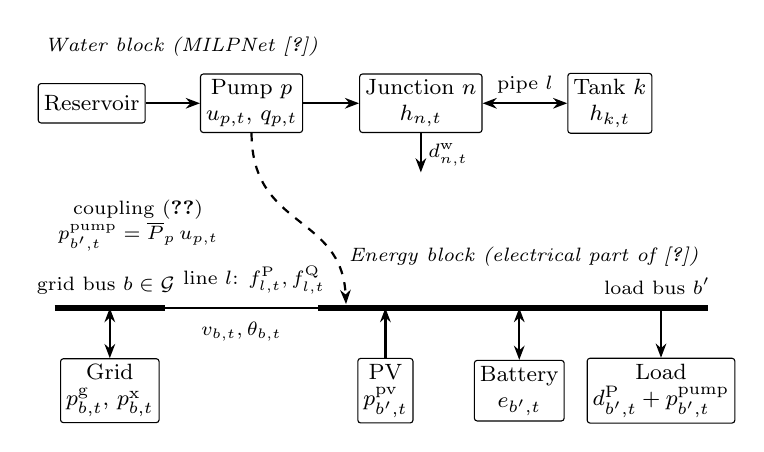
\begin{tikzpicture}[x=1cm,y=1cm,
  font=\footnotesize,
  >={Stealth[length=1.8mm]},
  box/.style={draw, rounded corners=1pt, minimum height=5mm, inner sep=2pt, align=center},
  wl/.style={draw=black, line width=0.8pt},
  el/.style={draw=black, line width=0.8pt},
  busl/.style={draw=black, line width=2.2pt},
]
% ---------------- water block ----------------
\node[font=\scriptsize\itshape, anchor=west] at (0.0,0.72) {Water block (MILPNet \cite{thomas2024})};
\node[box] (res) at (0.72,0) {Reservoir};
\node[box] (pump) at (2.75,0) {Pump $p$\\$u_{p,t},\,q_{p,t}$};
\node[box] (junc) at (4.9,0) {Junction $n$\\$h_{n,t}$};
\node[box] (tank) at (7.3,0) {Tank $k$\\$h_{k,t}$};
\draw[wl,->] (res) -- (pump);
\draw[wl,->] (pump) -- (junc);
\draw[wl,<->] (junc) -- node[above,font=\scriptsize]{pipe $l$} (tank);
\draw[wl,->] (junc.south) -- ++(0,-0.5) node[right=-1pt,pos=0.55,font=\scriptsize]{$d^{\mathrm{w}}_{n,t}$};
% ---------------- energy block ----------------
\node[font=\scriptsize\itshape, anchor=east] at (8.55,-1.95) {Energy block (electrical part of \cite{morvaj2016})};
\draw[busl] (0.25,-2.6) -- (1.65,-2.6);
\draw[busl] (3.6,-2.6) -- (8.55,-2.6);
\draw[el] (1.65,-2.6) -- (3.6,-2.6);
\node[font=\scriptsize, anchor=south] at (0.9,-2.55) {grid bus $b\in\Gset$};
\node[font=\scriptsize, anchor=south] at (7.9,-2.55) {load bus $b'$};
\node[font=\scriptsize, anchor=south] at (2.78,-2.55) {line $l$: $f^{\mathrm{P}}_{l,t},f^{\mathrm{Q}}_{l,t}$};
\node[font=\scriptsize, anchor=north] at (2.62,-2.65) {$v_{b,t},\theta_{b,t}$};
\node[box] (grid) at (0.95,-3.65) {Grid\\$p^{\mathrm{g}}_{b,t},\,p^{\mathrm{x}}_{b,t}$};
\draw[el,<->] (0.95,-2.6) -- (grid.north);
\node[box] (pv) at (4.45,-3.65) {PV\\$p^{\mathrm{pv}}_{b',t}$};
\node[box] (bat) at (6.15,-3.65) {Battery\\$e_{b',t}$};
\node[box] (load) at (7.95,-3.65) {Load\\$d^{\mathrm{P}}_{b',t}+p^{\mathrm{pump}}_{b',t}$};
\draw[el,->] (pv.north) -- (4.45,-2.6);
\draw[el,<->] (bat.north) -- (6.15,-2.6);
\draw[el,->] (7.95,-2.6) -- (load.north);
% ---------------- coupling ----------------
\draw[->, line width=0.8pt, dashed] (pump.south) .. controls (2.75,-1.6) and (3.9,-1.4) .. (3.95,-2.55);
\node[font=\scriptsize, align=center, anchor=east] at (2.45,-1.55) {coupling \eqref{eq:c_pumpload}\\$p^{\mathrm{pump}}_{b',t}=\overline{P}_p\,u_{p,t}$};
\end{tikzpicture}}
\caption{Coupled day-ahead scheduling problem. The water block and the energy block are imported from published MILP models; the only shared constraint is the pump electrical demand at its supply bus.}
\label{fig:system}
\end{figure}

The decision structure is that of a centralized benchmark: all network data and forecasts are available to one decision maker, and no bidding, contract, or decentralized coordination mechanism is modeled. The intended use is twofold: as an operational day-ahead schedule for a utility that owns both systems, and as the reference against which decentralized coordination schemes can be measured.

Table~\ref{tab:mapping} summarizes the constraints of the joint problem and their origin. Equations are numbered as they appear below; the source column refers to the equation numbers of \cite{thomas2024} (T\&S) and \cite{morvaj2016} (M).

\begin{table}[!t]
\caption{Constraints of the Joint Problem and Their Origin}
\label{tab:mapping}
\centering
\scriptsize
\setlength{\tabcolsep}{3pt}
\renewcommand{\arraystretch}{1.08}
\begin{tabular}{@{}p{2.9cm}p{1.45cm}p{3.75cm}@{}}
\toprule
Constraint & Source & Treatment in this paper \\
\midrule
\multicolumn{3}{@{}l}{\emph{Water block}}\\
Junction mass balance \eqref{eq:w_mass} & T\&S (1) & As published \\
Pipe energy conservation \eqref{eq:w_energy} & T\&S (2) & As published \\
Hazen--Williams loss \eqref{eq:w_hw} & T\&S (3) & PWL over a per-pipe signed domain \\
Tank dynamics \eqref{eq:w_tank} & T\&S (4) & Plus bounds and terminal reserve \\
Pump curve and status \eqref{eq:w_pumpcurve}--\eqref{eq:w_pumpM} & T\&S (5)--(7) & Status $1=$ on; closure slack eliminated \\
Gate valve \eqref{eq:w_gv} & T\&S (8), (11) & As published \\
PRV states \eqref{eq:w_prv} & T\&S (9), (12) & As published; not exercised \\
Tank-link checks, control rules & T\&S (13)--(15) & Omitted: statuses are decisions \\
Pressure floor \eqref{eq:w_pressure} & --- & Added service constraint \\
\midrule
\multicolumn{3}{@{}l}{\emph{Energy block}}\\
Electricity balance \eqref{eq:e_balance} & M (1), (14) & Nodal form; pump load added \\
Heat balance & M (2) & Omitted: no thermal coupling \\
Storage continuity \eqref{eq:e_soc} & M (3) & Efficiencies applied once \\
Capacity and exclusivity \eqref{eq:e_pv}--\eqref{eq:e_grid} & M, Sec.~2.2 & As described; terminal closure added \\
Linearized AC flow \eqref{eq:e_pflow}--\eqref{eq:e_qflow} & M (10), (11) & $U_0=1$~p.u. \\
Reactive balance \eqref{eq:e_qbalance} & M (15) & Grid supplies reactive power \\
Branch current \eqref{eq:e_ire}--\eqref{eq:e_thermal} & M (25)--(31) & SOS2 interpolation; no objective weight \\
Cost \eqref{eq:objective} & M (4) & Electricity streams only \\
\midrule
\multicolumn{3}{@{}l}{\emph{Coupling}}\\
Pump demand \eqref{eq:c_pumpload}, calibration \eqref{eq:c_calib} & --- & This paper \\
\bottomrule
\end{tabular}
\end{table}

\section{Water Distribution Block}
\label{sec:water}
The water block is the MILPNet formulation of Thomas and Sela \cite{thomas2024}. A directed graph contains junctions $\Jset$, tanks $\Kset$, reservoirs $\Rset$, and links $\Lset$ consisting of pipes $\Lpipe$, pumps $\Pset$, and valves $\Vset$. Link orientation fixes the sign of flow; pipes and gate valves may carry flow in either direction, whereas pumps do not allow backflow. Reservoir heads follow their prescribed time series, $h_{r,t}=H_{r,t}$ for $r\in\Rset$.

\subsection{Conservation Laws}
Mass balance at every junction and interval requires that the net inflow equal the demand \cite[Eq.~(1)]{thomas2024}:
\begin{equation}
\sum_{l\in\Lset}A^{\mathrm{w}}_{nl}\,q_{l,t}=d^{\mathrm{w}}_{n,t},\qquad n\in\Jset,\ t\in\Tset .
\label{eq:w_mass}
\end{equation}
Demand is the sum over all demand categories evaluated with the network's time patterns; consumption is demand driven, so pressure-dependent demand and leakage are not represented. Energy conservation along a pipe $l=(i,j)$ relates the head difference to the head loss \cite[Eq.~(2)]{thomas2024},
\begin{equation}
h_{i,t}-h_{j,t}-\Delta h_{l,t}=0,\qquad l\in\Lpipe,\ t\in\Tset ,
\label{eq:w_energy}
\end{equation}
and the head loss follows the Hazen--Williams relation \cite[Eq.~(3)]{thomas2024},
\begin{equation}
\Delta h_{l,t}=\sgn(q_{l,t})\,K_l\,|q_{l,t}|^{1.852},\qquad
K_l=\frac{10.67\,L_l}{C_l^{1.852}D_l^{4.8704}},
\label{eq:w_hw}
\end{equation}
with pipe length $L_l$ (m), diameter $D_l$ (m), and roughness $C_l$. Equation \eqref{eq:w_hw} is nonlinear and nonconvex because of the bidirectional flow, and MILPNet replaces it by a piecewise-linear (PWL) interpolation of the signed curve over a bounded flow domain. A service constraint that MILPNet leaves to the user is added here as a minimum pressure head at every junction:
\begin{equation}
h_{n,t}-z_n\geq\underline{\pi}_n,\qquad n\in\Jset,\ t\in\Tset .
\label{eq:w_pressure}
\end{equation}

\subsection{Piecewise-Linear Representation}
\label{sec:pwl}
All univariate nonlinearities in both blocks use the same construction. Given breakpoints $(x_s,y_s)$, $s=0,\dots,S$, with strictly increasing $x_s$, the relation $y=\pwl(x)$ is represented by nonnegative weights $\lambda_s$ and segment binaries $\delta_s$, $s=0,\dots,S-1$ \cite{bradley1977,beale1970,vielma2010}:
\begin{align}
x&=\sum_{s=0}^{S}\lambda_s x_s,\quad
y=\sum_{s=0}^{S}\lambda_s y_s,\quad
\sum_{s=0}^{S}\lambda_s=\sum_{s=0}^{S-1}\delta_s=\zeta,
\label{eq:pwl_interp}\\
\lambda_s&\leq\delta_{s-1}+\delta_s,\quad \delta_s\in\{0,1\},
\label{eq:pwl_adjacency}
\end{align}
where undefined end binaries are zero and $\zeta$ is an activation term. For pipes and lines $\zeta=1$; for a pump $\zeta=u_{p,t}$, so that both the flow and the head gain vanish when the pump is off. Adjacent breakpoints only can carry positive weight, which is the special-ordered-set (SOS2) condition written with explicit binaries; the formulation is therefore independent of solver-specific SOS or indicator support. For the Hazen--Williams curve, the breakpoints span a signed domain $[-\overline{q}_l,\overline{q}_l]$ with zero as a breakpoint; following MILPNet, the domain is set from an extended-period simulation of the network so that the segments cover the actual operating range. The interpolation is an equality surrogate of the nonlinear relation, not a relaxation with a guaranteed hydraulic error bound; the case study reports the resulting discrepancies through replay.

\subsection{Tanks and Inventory}
For a cylindrical tank $k$ the state is its total head, which evolves with the net inflow over each interval \cite[Eq.~(4)]{thomas2024}:
\begin{align}
h_{k,t+1}&=h_{k,t}+\frac{\dt_{\mathrm{s}}}{A_k}\sum_{l\in\Lset}A^{\mathrm{w}}_{kl}\,q_{l,t},
&&k\in\Kset,\ t\in\Tset,\label{eq:w_tank}\\
h_{k,0}&=h^0_k,\quad
\underline{h}_k\leq h_{k,t}\leq\overline{h}_k,
&&k\in\Kset,\ t\in\Tbar,\label{eq:w_tank_bounds}\\
h_{k,T}&\geq h^0_k,&&k\in\Kset .\label{eq:w_tank_terminal}
\end{align}
Two points distinguish \eqref{eq:w_tank}--\eqref{eq:w_tank_terminal} from a naive discretization. First, the inventory is defined on all $T+1$ boundaries, so the withdrawal or filling decided in the last interval changes $h_{k,T}$ and cannot disappear from the accounting. Second, the terminal condition \eqref{eq:w_tank_terminal} preserves the initial reserve, which prevents apparent savings obtained by draining the tank; all compared schedules must use the same terminal requirement. MILPNet's tank-link status checks \cite[Eq.~(13)]{thomas2024}, which reproduce the automatic closing of a tank inlet at full or empty conditions in a simulator, are replaced by the hard bounds \eqref{eq:w_tank_bounds}: a schedule that respects the bounds at every boundary does not trigger those checks in the discretized model, and whether it does so within an interval is a question for the replay of Section~\ref{sec:results}.

\subsection{Pumps}
A fixed-speed pump $p=(i,j)$ adds head according to a head--flow curve when it operates \cite[Eq.~(5)]{thomas2024}. MILPNet uses the quadratic form $a_p-b_pq^2$; EPANET's power-law form $g_p(q)=a_p-b_pq^{\nu_p}$ is used here so that single-point and three-point curves are covered by the same expression, and $g_p$ is interpolated over $[0,(a_p/b_p)^{1/\nu_p}]$ with the construction of Section~\ref{sec:pwl}:
\begin{equation}
\gamma_{p,t}=\pwl_p(q_{p,t})\ \text{with}\ \zeta=u_{p,t},\qquad p\in\Pset,\ t\in\Tset .
\label{eq:w_pumpcurve}
\end{equation}
MILPNet models the two states of a pump with a closure slack on the energy balance and a big-$M$ pair \cite[Eqs.~(6)--(7)]{thomas2024}. Eliminating the slack gives the equivalent form
\begin{align}
0\leq q_{p,t}&\leq\overline{q}_p\,u_{p,t},\label{eq:w_pumpflow}\\
-M_p(1-u_{p,t})&\leq h_{j,t}-h_{i,t}-\gamma_{p,t}\leq M_p(1-u_{p,t}),\label{eq:w_pumpM}
\end{align}
for $p\in\Pset$, $t\in\Tset$. When $u_{p,t}=1$ the downstream head equals the upstream head plus the curve gain; when $u_{p,t}=0$ the flow and the gain are zero and the two end heads are decoupled. The status convention is the complement of MILPNet's, where $y^t_p=0$ denotes an open pump; the convention used here makes the coupling term of Section~\ref{sec:coupling} a product of the status with a positive power. Finite flow and head bounds are needed both for physical interpretation and for valid constants $M_p$, which MILPNet sets just above the largest bound of the associated continuous variable.

\subsection{Valves}
Gate valves and pressure-reducing valves (PRVs) are retained from MILPNet for networks that contain them; the case study network has none, so these constraints are stated compactly. A gate valve $g=(i,j)$ with open status $y_{g,t}$ behaves like a pipe when open and disconnects its ends when closed \cite[Eqs.~(8), (11)]{thomas2024}:
\begin{equation}
\begin{aligned}
-\overline{q}_g\,y_{g,t}&\leq q_{g,t}\leq\overline{q}_g\,y_{g,t},\\
-M_g(1-y_{g,t})&\leq h_{i,t}-h_{j,t}-\Delta h_{g,t}\leq M_g(1-y_{g,t}),
\end{aligned}
\label{eq:w_gv}
\end{equation}
with $\Delta h_{g,t}$ the PWL Hazen--Williams loss of the valve. A PRV $v=(i,j)$ with setting $H^{\mathrm{set}}_v$ is in exactly one of three states, active ($\alpha_{v,t}$), open ($\omega_{v,t}$), or closed ($\kappa_{v,t}$) \cite[Eqs.~(9), (12)]{thomas2024}:
\begin{equation}
\begin{aligned}
&\alpha_{v,t}+\omega_{v,t}+\kappa_{v,t}=1,\qquad 0\leq q_{v,t}\leq\overline{q}_v(1-\kappa_{v,t}),\\
&|h_{j,t}-H^{\mathrm{set}}_v|\leq M_v(1-\alpha_{v,t}),\ \
h_{i,t}\geq H^{\mathrm{set}}_v-M_v(1-\alpha_{v,t}),\\
&|h_{i,t}-h_{j,t}|\leq M_v(1-\omega_{v,t}),\ \
h_{i,t}\leq H^{\mathrm{set}}_v+M_v(1-\omega_{v,t}),\\
&h_{i,t}-h_{j,t}+\epsilon\,\kappa_{v,t}\leq M_v(1-\kappa_{v,t}),
\end{aligned}
\label{eq:w_prv}
\end{equation}
where each absolute value denotes the corresponding pair of linear inequalities and $\epsilon>0$ replaces the strict inequality of the closed state, as in MILPNet. An active PRV holds its downstream head at the setting, an open PRV passes flow without additional loss, and a closed PRV blocks reverse flow.

\subsection{Control Rules}
MILPNet also formulates event-based and time-based control rules \cite[Eqs.~(14)--(15)]{thomas2024}, which make the MILP reproduce the rule-based behavior of an extended-period simulation. In the day-ahead scheduling problem the pump statuses are the decisions, so those rules are omitted; the rule-based schedule of the input file is used only for calibration (Section~\ref{sec:coupling}) and as an independent reference in the replay. MILPNet's pump-scheduling objective \cite[Eq.~(16)]{thomas2024} contains a fixed energy cost per operating hour and a switching penalty. The energy cost is replaced by the electrical coupling of Section~\ref{sec:coupling}; the switching penalty is not included in the present implementation, but it is linear in $u_{p,t}$ and can be added without changing the problem class.

\section{Distributed Energy System Block}
\label{sec:energy}
The energy block is the DES model of Morvaj \emph{et al.} \cite{morvaj2016}, whose energy-hub layer assigns conversion and storage technologies to meet electricity and heat demand while a linearized AC power-flow layer represents the distribution grid. Only the electrical part is imported. Each electrical bus $b\in\Bset$ hosts a hub with, at most, a PV generator, a battery, non-pump loads, and, if $b\in\Gset$, a grid connection. Conversion technologies with heat output and the thermal storage are absent, so the conversion-efficiency matrix of the hub reduces to the identity for PV and the heat balance \cite[Eq.~(2)]{morvaj2016} is dropped. The asset capacities are given, not designed.

\subsection{Electricity Balance}
The hub electricity balance \cite[Eq.~(1)]{morvaj2016} and the nodal active-power balance of the grid layer \cite[Eq.~(14)]{morvaj2016} are combined into one balance per bus, with the pump demand of Section~\ref{sec:coupling} added to the load:
\begin{multline}
p^{\mathrm{g}}_{b,t}-p^{\mathrm{x}}_{b,t}+p^{\mathrm{pv}}_{b,t}+p^{\mathrm{dis}}_{b,t}-p^{\mathrm{ch}}_{b,t}
+\sum_{l\in\Eset}A^{\mathrm{e}}_{bl}\,f^{\mathrm{P}}_{l,t}\\
=d^{\mathrm{P}}_{b,t}+p^{\mathrm{pump}}_{b,t},\qquad b\in\Bset,\ t\in\Tset .
\label{eq:e_balance}
\end{multline}
The reactive balance \cite[Eq.~(15)]{morvaj2016} is
\begin{equation}
r^{\mathrm{g}}_{b,t}+\sum_{l\in\Eset}A^{\mathrm{e}}_{bl}\,f^{\mathrm{Q}}_{l,t}=d^{\mathrm{Q}}_{b,t},\qquad b\in\Bset,\ t\in\Tset ,
\label{eq:e_qbalance}
\end{equation}
where PV, battery, and pump exchanges are at unity power factor and reactive load is supplied from the grid connection; $r^{\mathrm{g}}_{b,t}=0$ for $b\notin\Gset$. A non-unity pump power factor would add a term to \eqref{eq:e_qbalance} proportional to $p^{\mathrm{pump}}_{b,t}$.

\subsection{Storage, Generation, and Grid Exchange}
Storage continuity \cite[Eq.~(3)]{morvaj2016} is written with charging and discharging measured at the AC bus, so that the efficiencies appear once, in the inventory equation, and not again in the bus balance:
\begin{align}
e_{b,t+1}&=e_{b,t}+\dt\Big(\eta^{\mathrm{ch}}_b\,p^{\mathrm{ch}}_{b,t}-\frac{p^{\mathrm{dis}}_{b,t}}{\eta^{\mathrm{dis}}_b}\Big),
&&t\in\Tset,\label{eq:e_soc}\\
e_{b,0}&=e^0_b,\quad 0\leq e_{b,t}\leq\overline{e}_b,&&t\in\Tbar,\label{eq:e_soc_bounds}\\
e_{b,T}&\geq e^0_b .\label{eq:e_soc_terminal}
\end{align}
As for tanks, the inventory is tracked on all $T+1$ boundaries and the terminal energy must be replenished. PV can be curtailed within its availability,
\begin{equation}
0\leq p^{\mathrm{pv}}_{b,t}\leq\overline{p}^{\mathrm{pv}}_{b,t},
\label{eq:e_pv}
\end{equation}
and, as required in \cite{morvaj2016}, a storage cannot charge and discharge, nor can a bus import and export, in the same interval:
\begin{align}
0\leq p^{\mathrm{ch}}_{b,t}\leq\overline{p}^{\mathrm{ch}}_b y^{\mathrm{ch}}_{b,t},\ \
0\leq p^{\mathrm{dis}}_{b,t}\leq\overline{p}^{\mathrm{dis}}_b y^{\mathrm{dis}}_{b,t},\ \
y^{\mathrm{ch}}_{b,t}+y^{\mathrm{dis}}_{b,t}\leq1,\label{eq:e_battery_modes}\\
0\leq p^{\mathrm{g}}_{b,t}\leq\overline{p}^{\mathrm{g}} y^{\mathrm{g}}_{b,t},\ \
0\leq p^{\mathrm{x}}_{b,t}\leq\overline{p}^{\mathrm{x}} y^{\mathrm{x}}_{b,t},\ \
y^{\mathrm{g}}_{b,t}+y^{\mathrm{x}}_{b,t}\leq1,\label{eq:e_grid}
\end{align}
for $b\in\Bset$, $t\in\Tset$, with $p^{\mathrm{g}}_{b,t}=p^{\mathrm{x}}_{b,t}=0$ for $b\notin\Gset$ and zero storage and PV bounds at buses without those assets. Battery degradation is not modeled.

\subsection{Linearized AC Power Flow}
Each line $l=(i,j)$ has series impedance $R_l+\mathrm{j}X_l$ and series admittance $G_l+\mathrm{j}B_l$, with $G_l=R_l/(R_l^2+X_l^2)$ and $B_l=-X_l/(R_l^2+X_l^2)$. Morvaj \emph{et al.} adopt the linearization of \cite{koster2011}, a first-order expansion of the AC power-flow equations about a flat voltage profile $U_0$ with small angle differences \cite[Eqs.~(10)--(11)]{morvaj2016}. With $U_0=1$~p.u. and the power base $\SB$,
\begin{align}
f^{\mathrm{P}}_{l,t}&=\SB\big[G_l(v_{i,t}-v_{j,t})-B_l(\theta_{i,t}-\theta_{j,t})\big],\label{eq:e_pflow}\\
f^{\mathrm{Q}}_{l,t}&=\SB\big[-B_l(v_{i,t}-v_{j,t})-G_l(\theta_{i,t}-\theta_{j,t})\big],\label{eq:e_qflow}
\end{align}
for $l\in\Eset$, $t\in\Tset$. Voltage magnitudes obey $\underline{v}\leq v_{b,t}\leq\overline{v}$, and the reference bus has $v=1$ and $\theta=0$. The model is balanced, lossless, and topology fixed: each line has one signed flow whose receiving-end value is its negative, and shunt charging, transformer tap changes, phase imbalance, and higher-order terms are absent. A solution of \eqref{eq:e_pflow}--\eqref{eq:e_qflow} is therefore not a certificate of AC feasibility, which is why the optimized injections are replayed in a nonlinear power-flow solver in Section~\ref{sec:results}.

\subsection{Branch-Current Limits}
Distribution feeders are constrained by conductor ampacity as well as by voltage. Morvaj \emph{et al.} linearize the branch current by the same expansion, obtaining real and imaginary parts that are linear in the voltage and angle differences \cite[Eq.~(25)]{morvaj2016}. At the expansion point these components coincide with the per-unit line flows of \eqref{eq:e_pflow}--\eqref{eq:e_qflow}:
\begin{align}
i^{\re}_{l,t}&=G_l(v_{i,t}-v_{j,t})-B_l(\theta_{i,t}-\theta_{j,t})=f^{\mathrm{P}}_{l,t}/\SB,\label{eq:e_ire}\\
i^{\im}_{l,t}&=B_l(v_{i,t}-v_{j,t})+G_l(\theta_{i,t}-\theta_{j,t})=-f^{\mathrm{Q}}_{l,t}/\SB .\label{eq:e_iim}
\end{align}
The magnitude requires the sum of the squared components. Following \cite[Eqs.~(26)--(31)]{morvaj2016}, nonnegative auxiliary variables bound the absolute values,
\begin{equation}
\phi_{l,t}\geq\pm i^{\re}_{l,t},\qquad \chi_{l,t}\geq\pm i^{\im}_{l,t},
\label{eq:e_abs}
\end{equation}
their squares are interpolated on $[0,\overline{\imath}_l]$ with the construction of Section~\ref{sec:pwl}, and the interpolated squares are limited:
\begin{equation}
\hat\phi_{l,t}=\pwl(\phi_{l,t}^2),\quad
\hat\chi_{l,t}=\pwl(\chi_{l,t}^2),\quad
\hat\phi_{l,t}+\hat\chi_{l,t}\leq\overline{\imath}_l^{\,2}.
\label{eq:e_thermal}
\end{equation}
Two details differ from \cite{morvaj2016}. There, the absolute values are pushed toward the current components by a small objective weight, and the convexity of $x^2$ makes the SOS2 adjacency condition unnecessary. Here the adjacency binaries of \eqref{eq:pwl_adjacency} are kept, so the same interpolation code serves both blocks, and no objective perturbation is needed: increasing $\phi_{l,t}$ or $\chi_{l,t}$ beyond the absolute value can only tighten \eqref{eq:e_thermal}, so any feasible schedule remains feasible with $\phi_{l,t}=|i^{\re}_{l,t}|$ and $\chi_{l,t}=|i^{\im}_{l,t}|$. Because each secant lies above $x^2$, the constraint is conservative for the magnitude of the linearized current, with a maximum interpolation excess of $\Delta x^2/4$ on a segment of width $\Delta x$; finer segments reduce this conservatism at the cost of more binaries but do not correct the error of the underlying linearization.

\section{Coupling and the Day-Ahead MILP}
\label{sec:coupling}
\subsection{Pump Electrical Demand}
The two blocks share one constraint. Each running pump draws a constant electrical power $\overline{P}_p$ at the bus that supplies it, and the demand at bus $b$ is
\begin{equation}
p^{\mathrm{pump}}_{b,t}=\sum_{p\in\Pset_b}\overline{P}_p\,u_{p,t},\qquad b\in\Bset,\ t\in\Tset ,
\label{eq:c_pumpload}
\end{equation}
which enters the bus balance \eqref{eq:e_balance}. The coefficient is calibrated from an extended-period EPANET simulation of the input network under its original controls, the same simulation that MILPNet uses to bound the PWL domains. With $q^{\mathrm{sim}}_{p,\tau}$ and $\Delta h^{\mathrm{sim}}_{p,\tau}$ the simulated flow and head gain of pump $p$, and $\mathcal{O}_p$ the set of simulation steps in which it runs,
\begin{equation}
\overline{P}_p=\frac{\rho g}{\eta_p}\cdot\frac{1}{|\mathcal{O}_p|}\sum_{\tau\in\mathcal{O}_p}q^{\mathrm{sim}}_{p,\tau}\,\Delta h^{\mathrm{sim}}_{p,\tau},
\label{eq:c_calib}
\end{equation}
with $\rho g=9.81$~kW$\cdot$s/m$^4$ for water. Equation \eqref{eq:c_pumpload} is linear in the existing pump status, so the coupled problem introduces no new nonlinearity or integrality. It is also the principal coupling approximation: the modeled electrical draw depends on whether the pump runs, not on the optimized flow and head. Its consequences are examined in Sections~\ref{sec:results} and~\ref{sec:discussion}.

\subsection{Objective}
The DES objective of \cite[Eq.~(4)]{morvaj2016} is a weighted sum of input energy streams. With natural gas absent and the weights equal to day-ahead prices, it reduces to the electricity procurement cost net of export revenue:
\begin{equation}
\min\ C=\dt\sum_{t\in\Tset}\sum_{b\in\Gset}\big(c^{\mathrm{buy}}_t\,p^{\mathrm{g}}_{b,t}-c^{\mathrm{sell}}_t\,p^{\mathrm{x}}_{b,t}\big).
\label{eq:objective}
\end{equation}
Pumping enters \eqref{eq:objective} only through \eqref{eq:c_pumpload} and \eqref{eq:e_balance}, so it is charged once; the fixed per-hour pump cost of MILPNet's scheduling objective is removed to avoid double counting. No artificial water-flow cost is added.

\subsection{Complete Problem and Properties}
The day-ahead coordinated scheduling problem is
\begin{equation}
\begin{aligned}
\min\quad & C \text{ in \eqref{eq:objective}}\\
\text{s.t.}\quad & \text{water block: } \eqref{eq:w_mass}\text{--}\eqref{eq:w_pressure},\ \eqref{eq:w_tank}\text{--}\eqref{eq:w_prv},\\
& \text{energy block: } \eqref{eq:e_balance}\text{--}\eqref{eq:e_thermal},\\
& \text{coupling: } \eqref{eq:c_pumpload},\\
& \text{PWL relations: } \eqref{eq:pwl_interp}\text{--}\eqref{eq:pwl_adjacency},\quad
u,y,\alpha,\omega,\kappa,\delta\in\{0,1\}.
\end{aligned}
\label{eq:milp}
\end{equation}
Problem \eqref{eq:milp} is a MILP. Its binaries are the pump statuses, valve states, storage and grid modes, and the PWL segment selectors; all other variables are continuous. Three properties follow directly from the construction. First, tanks and batteries have the same accounting role: each can move consumption across time but neither can supply net energy or water through an unrecorded terminal withdrawal, because of \eqref{eq:w_tank_terminal} and \eqref{eq:e_soc_terminal}. Second, with exact solves, fixing the pump statuses to any feasible schedule cannot decrease the optimal cost, so the difference between a fixed-schedule solve and the joint solve is a nonnegative measure of the value of coordination under identical assumptions; a violation of this ordering indicates unequal assumptions, a solver gap, or a reporting error rather than negative flexibility. Third, if the demand balance \eqref{eq:w_mass} is relaxed with slacks $s^{\pm}_{n,t}$ and a large penalty for diagnosis, any nonzero slack is a service violation and must be reported as such; the results below use the exact balance.

\section{Implementation and Experimental Protocol}
\label{sec:implementation}
\subsection{Workflow}
The formulation is implemented in Python with Pyomo \cite{pyomo2011,pyomo2021} as a shared model assembled from optional water and energy components (Fig.~\ref{fig:workflow}). EPANET input files are read through WNTR \cite{klise2017}, and buses, loads, line parameters, and base quantities are extracted from an OpenDSS circuit \cite{dugan2011}. A configuration file specifies the horizon, assets, tariffs, pump-to-bus assignments, PWL segment counts, bounds, and solver options, which separates the physical network description from the economic experiment. The workflow validates the configuration, runs the EPANET calibration simulation that supplies the PWL flow domains and the pump coefficients \eqref{eq:c_calib}, builds the MILP, solves it, checks solver status and the presence of an incumbent before extracting a solution, and writes schedules, inventories, and summary metrics. The case study was solved with Gurobi 12.0.3 \cite{gurobi} through Pyomo 6.9.4 at a relative optimality gap tolerance of $10^{-4}$; the open-source solver HiGHS \cite{huangfu2018} is supported as well. Dependency versions and hashes of the source and input files are recorded with every run.

\begin{figure}[!t]
\centering
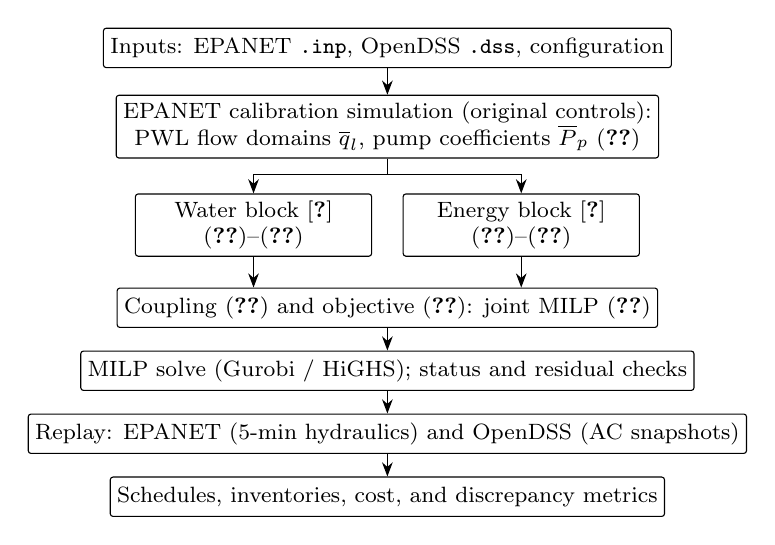
\begin{tikzpicture}[x=1cm,y=1cm,
  font=\footnotesize, >={Stealth[length=1.8mm]},
  stage/.style={draw, rounded corners=1pt, minimum width=64mm, minimum height=5mm, inner sep=2.5pt, align=center},
  side/.style={draw, rounded corners=1pt, minimum width=30mm, minimum height=5mm, inner sep=2.5pt, align=center},
]
\node[stage] (in) at (0,0) {Inputs: EPANET \texttt{.inp}, OpenDSS \texttt{.dss}, configuration};
\node[stage] (sim) at (0,-1.0) {EPANET calibration simulation (original controls):\\PWL flow domains $\overline{q}_l$, pump coefficients $\overline{P}_p$ \eqref{eq:c_calib}};
\node[side] (w) at (-1.7,-2.25) {Water block \cite{thomas2024}\\\eqref{eq:w_mass}--\eqref{eq:w_prv}};
\node[side] (e) at (1.7,-2.25) {Energy block \cite{morvaj2016}\\\eqref{eq:e_balance}--\eqref{eq:e_thermal}};
\node[stage] (c) at (0,-3.3) {Coupling \eqref{eq:c_pumpload} and objective \eqref{eq:objective}: joint MILP \eqref{eq:milp}};
\node[stage] (solve) at (0,-4.1) {MILP solve (Gurobi / HiGHS); status and residual checks};
\node[stage] (rep) at (0,-4.9) {Replay: EPANET (5-min hydraulics) and OpenDSS (AC snapshots)};
\node[stage] (out) at (0,-5.7) {Schedules, inventories, cost, and discrepancy metrics};
\draw[->] (in) -- (sim);
\draw[->] (sim.south) -- ++(0,-0.2) -| (w.north);
\draw[->] (sim.south) -- ++(0,-0.2) -| (e.north);
\draw[->] (w.south) -- (w.south |- c.north);
\draw[->] (e.south) -- (e.south |- c.north);
\draw[->] (c) -- (solve);
\draw[->] (solve) -- (rep);
\draw[->] (rep) -- (out);
\end{tikzpicture}
\caption{Implementation workflow. Calibration and diagnostic linearizations are separated from the piecewise-linear scheduling formulation, and MILP feasibility is separated from nonlinear replay.}
\label{fig:workflow}
\end{figure}

\subsection{Comparison Protocol}
The experiment asks whether choosing pump operation jointly with electrical dispatch changes the procurement cost relative to a feasible pumping schedule selected without regard to the electrical system, under the same asset availability and tariff. The independent baseline is constructed in two steps: the water block alone is solved with a uniform pump energy price, which yields an energy-efficient schedule as a water operator would select without price information; that schedule is then fixed in the joint model and the electrical dispatch is optimized under the time-varying prices. Joint scheduling releases the pump binaries and optimizes the same objective with identical network, asset, initial-inventory, and terminal constraints. A flat-price joint case serves as a tariff sensitivity. Only within-tariff comparisons with identical constraints estimate the scheduling benefit; the difference between bills under two tariffs combines an operating response with a price change, and a comparison with and without a battery measures both an asset change and its scheduling. A uniform-price water objective can admit several optimal pumping schedules, so the reported benefit is relative to the particular recorded baseline schedule, not an average over uncoordinated policies.

\subsection{Replay}
Solver feasibility, formulation tests, and physical replay answer different questions. Unit and integration tests establish that the constraints conserve inventory, enforce asset limits, preserve units, and route the pump demand to the correct bus. Algebraic residuals of the solved MILP establish consistency with the implemented surrogate. Replaying the optimized decisions in independent nonlinear simulators assesses physical fidelity on the instance. In the replay, the optimized pump statuses are imposed on the original EPANET network with a five-minute hydraulic time step and hourly reports, and the optimized net bus injections, including PV, storage, and pump power, are solved as balanced constant-power snapshots in OpenDSS. Agreement obtained after fixing variables at a simulator's operating point would only be a consistency check; the replay reported here assesses the proposed schedules themselves.

\section{Case Study}
\label{sec:results}
\IfFileExists{results.tex}{\subsection{Test System and Data}
The water operator runs the SNET network of the repository: one ground-level reservoir, one fixed-speed pump
(design point 50~L/s at 40~m, wire-to-water efficiency 0.75, calibrated on-state power $\overline{P}_p=25.95$~kW),
two junctions, two pipes, and one elevated cylindrical tank (12~m diameter, 25~m
elevation, level 0--6~m, initial 3~m). Daily
demand is 2,214~m$^3$ with the diurnal pattern of Fig.~\ref{fig:inputs}; a 20~m pressure
floor and terminal replenishment are enforced. The tank holds about 2.8 pump-hours of water, so
the shiftable volume is tank-limited in the sense of the two-period model. The energy operator owns the two-bus feeder of the
repository with its daily load shape scaled to a 100~kW peak, a 200~kW$_\mathrm{p}$
PV array, a 200~kWh/50~kW battery ($\eta=0.95$, initial and minimum terminal energy 100~kWh), and a connection rated
150~kW import and 50~kW export. Day-ahead purchase prices are 0.08 in hours 0, 1, 2, 3, 4, 5, 6, 21, 22, and 23; 0.16 in hours 7, 8, 9, 10, 11, 12, 13, 14, and 15; 0.32 in hours 16, 17, 18, 19, and 20
(unit/kWh); the sale price is 0.03. The flat retail tariff of the baseline is $\bar\tau=0.16$, the
time average of the purchase price. Profiles are synthetic and illustrative (Table~\ref{tab:case}).

\begin{table}[!t]
\caption{Case-Study Data (Synthetic Profiles, One-Hour Intervals)}
\label{tab:case}
\centering
\footnotesize
\setlength{\tabcolsep}{4pt}
\begin{tabular}{@{}lp{5.4cm}@{}}
\toprule
Item & Value \\
\midrule
Water network & SNET: 1 reservoir, 1 pump, 2 junctions, 2 pipes, 1 tank \\
Tank & 12~m diameter, elevation 25~m, level 0--6~m, initial 3~m \\
Demand, pressure floor & 2,214~m$^3$/day with daily pattern; 20~m \\
Pump & 50~L/s at 40~m; $\eta_p=0.75$; $\overline{P}_p=25.95$~kW; 6 PWL segments \\
Pipes, line currents & 12 PWL segments (signed domain), 5 segments \\
Feeder & Two-bus circuit, load shape peaking at 100~kW \\
PV, battery & 200~kW$_\mathrm{p}$; 200~kWh, 50~kW, $\eta=0.95$, $e^0=100$~kWh \\
Connection & 150~kW import, 50~kW export; $0.9\le v\le1.1$~p.u. \\
Prices (unit/kWh) & purchase 0.08/0.16/0.32 (off/mid/on-peak); sale 0.03; flat tariff 0.16 \\
\bottomrule
\end{tabular}
\end{table}

\begin{figure}[!t]
\centering
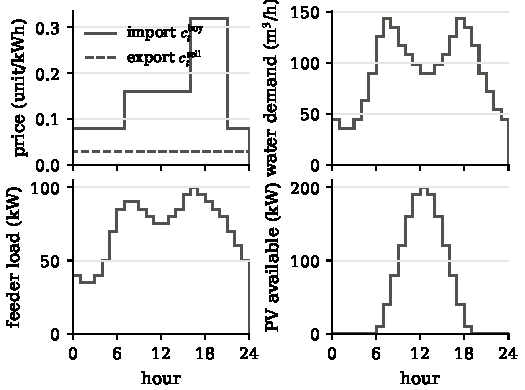
\includegraphics[width=\columnwidth]{inputs.pdf}
\caption{Input profiles: day-ahead purchase and sale prices, water demand, feeder load, and available PV power.}
\label{fig:inputs}
\end{figure}

\subsection{Experiments}
Six experiments are run: (E1) the flat-tariff baseline and the two tariff benchmarks against the integrated optimum;
(E2) the payoffs of the revenue-sharing contract, the fee window, and a numerical deviation test; (E3) the replay of the
baseline and coordinated schedules in EPANET and OpenDSS; (E4) the price coordination scheme with the bundle
master started from the energy operator's marginal costs and from the market price, and with the subgradient rule of the two-agent model; (E5) sweeps of the import and export
ratings of the connection; and (E6) the restricted-LP internal prices that verify Proposition~\ref{prop:price}.
All models were solved with HiGHS 1.11.0 through Pyomo; the integrated MILP has 3219
variables and 2598 constraints and was solved to a 0.003\% relative gap in
76~s, the coordination subproblems to a 0.1\% gap. Timing includes the
Pyomo interface overhead and is not a solver benchmark.

\subsection{The Value of Coordination (E1, E6)}
Table~\ref{tab:arrangements} compares the arrangements. Under the flat tariff the water operator needs
9 pump-hours and, holding its level, places 2~h at 0.08, 5~h at 0.16, 2~h at 0.32 (unit/kWh);
the site's day-ahead cost is 107.94/day. The integrated optimum pumps 3~h at 0.08, 6~h at 0.16, 0~h at 0.32 and costs 90.91/day,
a coordination gain $\mathcal{G}=17.03$/day, 15.8\% of the site's bill and
46\% of the water operator's baseline pumping bill of 37.37/day.
Figure~\ref{fig:computed} shows how the gain is earned: the coordinated schedule places 5 of its 9 pump-hours in the export and idle hours, where the site's own energy is cheapest, and none in the peak block at 0.32; the baseline, holding its level, places 4 in the surplus hours and 2 in the peak block, which the grid serves at the peak price.

The internal price $\pi^\star_t$ of the restricted LP follows Proposition~\ref{prop:price}: in the 15 hours in which the site imports it equals the purchase price; in the 6 export hours (hours 9, 10, 11, 12, 13, and 14) it equals the sale price 0.03; in the 3 idle hours (hours 7, 8, and 16) it lies inside the band $[c^{\mathrm{sell}}_t, c^{\mathrm{buy}}_t]$, set by the battery's intertemporal arbitrage. Passing the purchase price through to the water operator captures 95.6\% of the gain: the water operator then avoids the peak block but places only 5 pump-hours in the surplus hours, having no reason to prefer them over the other hours of the same purchase price. Charging the internal price itself captures 98.2\%: the water operator is indifferent among equally priced hours, and the tie it happened to break is not the one the energy operator can serve most cheaply (Proposition~\ref{prop:tariff}).

\begin{table}[!t]
\caption{Arrangements Compared (Unit/Day). Gain and Capture Are Relative to the Baseline}
\label{tab:arrangements}
\centering
\scriptsize
\setlength{\tabcolsep}{2pt}
\begin{tabular}{@{}lrrrrrr@{}}
\toprule
Arrangement & Cost & Gain & Capt.\ (\%) & On (h) & Import & Export \\
\midrule
Baseline: flat tariff, level holding & 107.94 & 0.00 & 0.0 & 9 & 856 & 212 \\
Pass-through tariff $\tau_t=c^{\mathrm{buy}}_t$ & 91.66 & 16.28 & 95.6 & 9 & 830 & 201 \\
Internal-price tariff $\tau_t=\pi^\star_t$ & 91.21 & 16.73 & 98.2 & 9 & 830 & 216 \\
Integrated optimum (contract) & 90.91 & 17.03 & 100.0 & 9 & 830 & 226 \\
\bottomrule
\end{tabular}
\end{table}

\begin{figure}[!t]
\centering
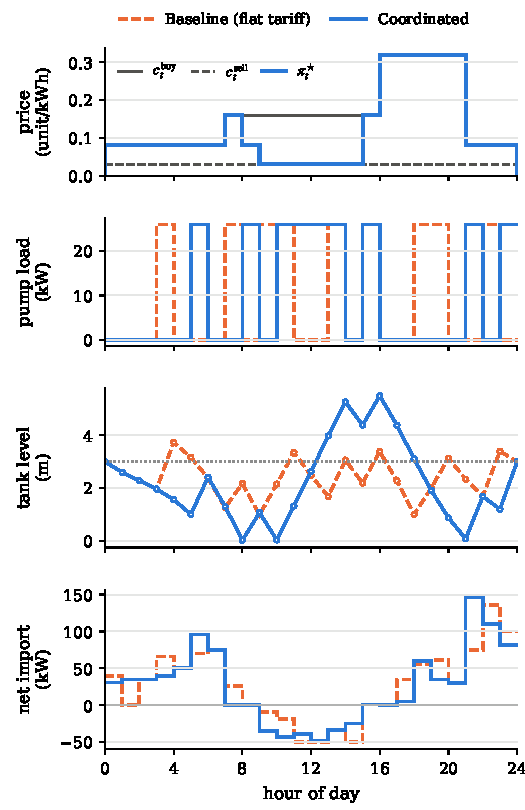
\includegraphics[width=\columnwidth]{coordination_results.pdf}
\caption{Baseline versus coordinated operation. Top to bottom: purchase and sale prices with the internal price
$\pi^\star_t$; pump load; tank level (markers are inventory boundaries, the dotted line the initial level); net import
at the connection (negative is export).}
\label{fig:computed}
\end{figure}

\subsection{Dividing the Gain (E2)}
Table~\ref{tab:payoffs} lists the payoffs. Because the site is a net importer, the settlement is negative
($R^\star=-90.91$/day), and the contract is read as bill sharing: with the fee anchored on the baseline,
$F(\varphi)=\mathrm{bill}^0+\varphi R^0$, the water operator's payoff rises by $\varphi\mathcal{G}$ and the energy
operator's by $(1-\varphi)\mathcal{G}$ at every share (Corollary~\ref{cor:window}). At the equal split $\varphi=1/2$
the fee is -16.60/day and each operator gains 8.51/day; for that share any fee in
$[-25.11,\,-8.09]$ leaves both operators no worse off than the baseline, an interval of width
$\mathcal{G}$. The deviation test in Table~\ref{tab:deviation} evaluates the water operator's contract payoff at
$\varphi=1/2$ if it ran one of the other schedules instead, with the energy operator responding optimally: every
deviation loses, as Theorem~\ref{thm:contract} requires.

\begin{table}[!t]
\caption{Daily Payoffs by Arrangement (Unit/Day); Fee Anchored on the Baseline}
\label{tab:payoffs}
\centering
\scriptsize
\setlength{\tabcolsep}{2.5pt}
\begin{tabular}{@{}lrrrrrrr@{}}
\toprule
Arrangement & $\varphi$ & $F$ & $\Pi_{\mathrm{W}}$ & $\Pi_{\mathrm{E}}$ & $\Pi$ & $\Delta\Pi_{\mathrm{W}}$ & $\Delta\Pi_{\mathrm{E}}$ \\
\midrule
Baseline (flat tariff) & -- & -- & -37.37 & -70.57 & -107.94 & -- & -- \\
Contract & 0.00 & 37.37 & -37.37 & -53.54 & -90.91 & +0.00 & +17.03 \\
Contract & 0.50 & -16.60 & -28.85 & -62.05 & -90.91 & +8.51 & +8.51 \\
Contract & 1.00 & -70.57 & -20.34 & -70.57 & -90.91 & +17.03 & +0.00 \\
\bottomrule
\end{tabular}
\end{table}

\begin{table}[!t]
\caption{Water Operator's Contract Payoff at $\varphi=1/2$ for Alternative Schedules (Unit/Day)}
\label{tab:deviation}
\centering
\footnotesize
\setlength{\tabcolsep}{4pt}
\begin{tabular}{@{}lrr@{}}
\toprule
Schedule run by W & $\Pi_{\mathrm{W}}$ & Deviation gain \\
\midrule
Baseline: flat tariff, level holding & -37.37 & -8.51 \\
Pass-through tariff $\tau_t=c^{\mathrm{buy}}_t$ & -29.23 & -0.38 \\
Internal-price tariff $\tau_t=\pi^\star_t$ & -29.00 & -0.15 \\
Integrated optimum (contract) & -28.85 & +0.00 \\
\bottomrule
\end{tabular}
\end{table}

\subsection{Distributed Computation (E4)}
Table~\ref{tab:coordination} and Fig.~\ref{fig:convergence} summarize the price coordination runs. Started from the
energy operator's marginal cost of serving the metered baseline schedule, the first message of the recommended protocol, the
scheme certifies a gap of 0.72\% after the first exchange, the recovered schedule attains the
integrated optimum at iteration 2, and the bundle master stops after 7 iterations, when its model
predicts no further improvement at the exchanged price resolution, with a dual bound of 90.55/day and a
certified gap of 0.39\%. Started from the market price instead, the first exchange certifies only
8.18\%, because the purchase price leaves the energy operator indifferent in every import hour;
the scheme attains the optimum at iteration 7, reaches a 1\% certificate at iteration 17,
and ends after 29 iterations with a gap of 0.02\%. The subgradient rule from the
marginal-cost start attains the optimum at iteration 2 and reaches a gap of 0.39\% after
15 iterations. Evaluating the dual function at the restricted-LP prices $\pi^\star$ gives $D(\pi^\star)=90.91$/day against $C^\star=90.91$/day: the Lagrangian relaxation of the interface has no duality gap on this instance (Proposition~\ref{prop:convergence}(iv)), so the residual certified gap of the runs is the price of finite iterations, quantized prices, and subproblem tolerances, not a structural limit. For comparison, the central solver's own bound on the integrated MILP is
90.90, a gap of 0.003\%, and it holds both operators' data. Each iteration exchanges 48 scalars; no demand forecast, tank state, pump
characteristic, PV forecast, battery state, or market position crosses the boundary.

\begin{table}[!t]
\caption{Price Coordination Runs: Iterations, Messages, Certified Dual and Primal Values, Final Gap, the Iteration at Which the Recovered Schedule First Attains the Integrated Optimum, and Wall Time}
\label{tab:coordination}
\centering
\scriptsize
\setlength{\tabcolsep}{2pt}
\begin{tabular}{@{}lrrrrrrr@{}}
\toprule
Run & Iter. & Msgs & Dual & Primal & Gap \% & Opt.\ at & Min \\
\midrule
Bundle, marginal-cost start & 7 & 336 & 90.55 & 90.91 & 0.39 & 2 & 4.5 \\
Bundle, market-price start & 29 & 1392 & 90.89 & 90.91 & 0.02 & 7 & 57.2 \\
Subgradient, marginal-cost start & 15 & 720 & 90.55 & 90.91 & 0.39 & 2 & 10.7 \\
\bottomrule
\end{tabular}
\end{table}

\begin{figure*}[!t]
\centering
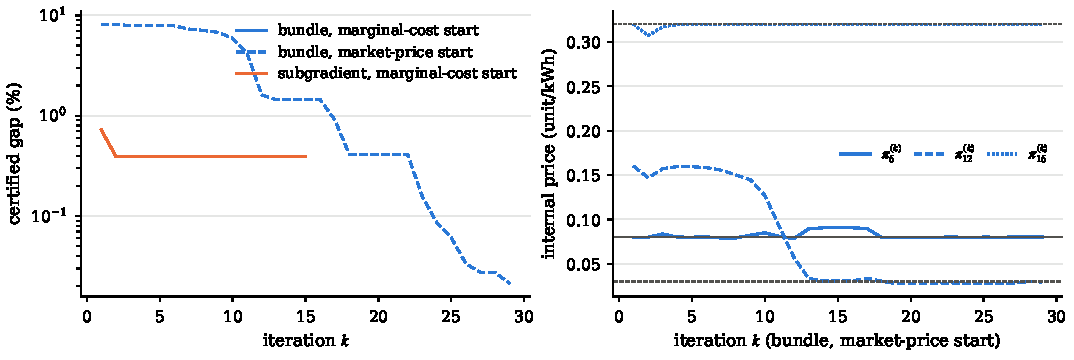
\includegraphics[width=\textwidth]{convergence.pdf}
\caption{Left: certified gap between the recovered primal value and the certified dual bound per iteration for the bundle
master from the marginal-cost and market-price starts and for the subgradient rule. Right: internal-price iterates at three
hours for the bundle run from the market-price start; thin lines mark the restricted-LP prices $\pi^\star_t$.}
\label{fig:convergence}
\end{figure*}

\subsection{Connection-Limit Sensitivities (E5)}
Table~\ref{tab:sweep} and Fig.~\ref{fig:sensitivity} vary the ratings of the connection. Tightening the import rating lowers the gain from 17.03/day at 150~kW to 10.92/day at 70~kW; at 100~kW and below the internal price departs from the market price in hours 21, 22, and 23, where the rating binds. No schedule is feasible at 60~kW. Tightening the export rating lowers the gain from 17.03/day at 50~kW to 16.61/day at 0~kW: with less room to export, both schedules absorb more of the midday surplus on site, and the internal price in the curtailment hours falls to the marginal value of spilled energy, zero, for the coordinated schedule and the baseline alike.

\begin{table}[!t]
\caption{Connection-Limit Sweeps (Unit/Day). ``Off Reference'' Lists the Non-Idle Hours in Which the Internal Price Departs from the Market Price of the Connection's Direction}
\label{tab:sweep}
\centering
\footnotesize
\setlength{\tabcolsep}{3pt}
\begin{tabular}{@{}lrrrrp{2.2cm}@{}}
\toprule
Limit & kW & Baseline & Integrated & Gain & Off reference \\
\midrule
Import & 150 & 107.94 & 90.91 & 17.03 & none \\
Import & 125 & 107.94 & 90.91 & 17.03 & none \\
Import & 100 & 110.28 & 98.67 & 11.61 & hours 21, 22, and 23 \\
Import & 90 & 116.54 & 105.12 & 11.43 & hours 21, 22, and 23 \\
Import & 80 & 122.99 & 111.75 & 11.24 & hours 5, 21, 22, and 23 \\
Import & 70 & 129.57 & 118.64 & 10.92 & hours 5, 6, 21, 22, and 23 \\
Import & 60 & infeasible & infeasible & -- & -- \\
Export & 50 & 107.94 & 90.91 & 17.03 & none \\
Export & 25 & 110.26 & 93.18 & 17.09 & hours 9, 10, 11, 12, 13, and 14 \\
Export & 0 & 114.29 & 97.68 & 16.61 & none \\
\bottomrule
\end{tabular}
\end{table}

\begin{figure*}[!t]
\centering
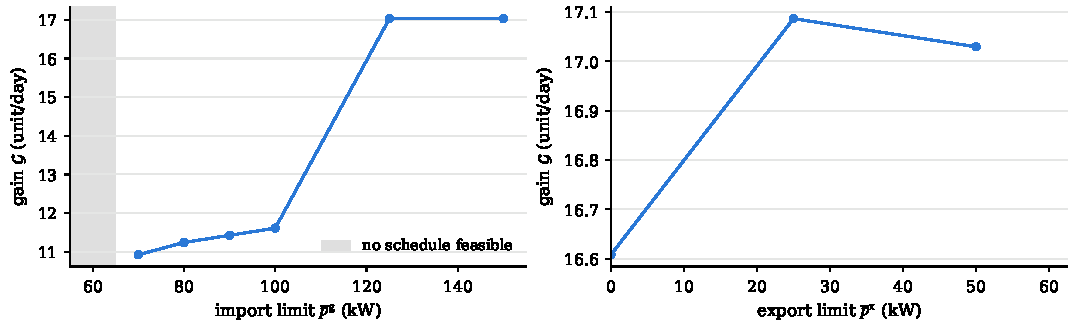
\includegraphics[width=\textwidth]{sensitivity.pdf}
\caption{Coordination gain versus the import rating (left) and the export rating (right) of the connection. Shaded bands
mark ratings at which only coordinated operation is feasible or no schedule is feasible.}
\label{fig:sensitivity}
\end{figure*}

\subsection{Independent Nonlinear Replay (E3)}
The baseline and coordinated pump schedules are replayed in EPANET with a five-minute hydraulic time step and hourly
reports, the level controls of the input file being replaced by the hourly commands, and the optimized net bus injections
are solved as balanced constant-power snapshots in OpenDSS. Table~\ref{tab:replay} summarizes the discrepancies.
Both schedules satisfy the pressure floor and the voltage band at every report time and the imposed pump statuses match the
MILP decisions. The replay ends with the tank 0.137~m (baseline) and 0.124~m (coordinated) below its initial level despite the replenishment constraint \eqref{eq:w_tank_terminal}, so the hourly hydraulic approximation does not preserve the terminal requirement exactly. The electrical discrepancies are small because the feeder is short and lightly loaded,
the regime in which the flat-voltage linearization is most accurate. Report-time checks do not certify feasibility between
reports; the results support the schedules as planning-stage outputs, not as a certification for field operation.

\begin{table}[!t]
\caption{Replay of the Baseline and Coordinated Schedules in EPANET and OpenDSS}
\label{tab:replay}
\centering
\footnotesize
\setlength{\tabcolsep}{4pt}
\begin{tabular}{@{}lrr@{}}
\toprule
Metric & Baseline & Coordinated \\
\midrule
Minimum junction pressure (m) & 25.92 & 25.03 \\
Pressure violations at report times & 0 & 0 \\
Pump-status mismatches at report times & 0 & 0 \\
Maximum tank-head discrepancy (m) & 0.139 & 0.125 \\
Maximum flow discrepancy (L/s) & 0.350 & 0.374 \\
Terminal tank-head change vs.\ initial (m) & $-0.137$ & $-0.124$ \\
All OpenDSS snapshots converged & yes & yes \\
Maximum voltage discrepancy (p.u.) & 0.00002 & 0.00003 \\
Voltage violations & 0 & 0 \\
Peak line loading (\%) & 0.17 & 0.19 \\
Maximum grid-exchange discrepancy (kW) & 0.000 & 0.000 \\
\bottomrule
\end{tabular}
\end{table}
}{%
The numerical-results file is not present in this checkout. Run \texttt{python -m src.experiments} from the repository root to generate \texttt{paper/results.tex} and the associated figure before using this manuscript as a completed empirical report.
}

\section{Discussion and Limitations}
\label{sec:discussion}
The computed cost difference arises from timing rather than from reduced electricity use: the independent and joint schedules have the same total import and the same pump on-hours, and the joint schedule removes the single pumping hour that the baseline placed in the peak tariff block. The small relative saving should be read against the modest pump load compared with the feeder's non-pump demand and against the lightly loaded feeder, which does not let the experiment demonstrate congestion relief. The absolute mechanism, however, is exactly what the formulation is meant to capture: within the hydraulic feasible set defined by the water block, pumping moves to the hours in which the energy block finds electricity cheapest.

The fixed on-state pump coefficient \eqref{eq:c_calib} is the principal coupling approximation. It keeps the interface linear and makes the effect of pump timing directly visible, but it can favor schedules whose simulated flow and head depart from the calibration trajectory, and it does not reward operating a pump near its best-efficiency point. Modeled pump-energy savings are savings under that coefficient until replay flows and heads are converted to electrical consumption; the electrical replay in this study keeps the same coefficient and therefore assesses the feeder approximation, not the pump-energy model. A validated PWL relation between electrical pump power and the hydraulic operating point is the natural next step, and variable-speed pumps would require speed-dependent characteristics, both of which MILPNet's device structure can accommodate.

The terminal reserve shortfall observed in the hydraulic replay is a second consequence of the hourly discretization. Tank dynamics \eqref{eq:w_tank} constrain interval-end volumes with interval-average flows, whereas the simulator resolves within-hour head changes and the resulting variation of pump flow along its curve. A reserve margin above $h^0_k$, a shorter interval, or a simulation-informed correction of the tank equation would close the gap; whichever is chosen, all compared schedules must share it.

Further limitations bound the numerical evidence. A small synthetic water network and a two-bus circuit do not establish scalability, performance under congestion, or behavior on real operator data. Coarse hydraulic interpolation can bias pressures and volumes, and flow domains derived from a reference schedule can exclude feasible operation outside that domain. The linearized power flow is most defensible near its flat-voltage expansion point, and the conservatism of \eqref{eq:e_thermal} does not compensate for its error. Hourly decisions miss sub-hourly tank-control events, motor starts, and short voltage excursions. Water quality, leakage, battery wear, pump switching costs, equipment outages, and forecast uncertainty are absent. Finally, the centralized decision structure assumes that one operator owns both systems; where the water and energy operators are distinct entities with private information, \eqref{eq:milp} is the benchmark that a decentralized coordination mechanism should approach, not a description of how such operators would actually interact.

\section{Conclusion}
\label{sec:conclusion}
This paper formulated the day-ahead coordinated scheduling of a water distribution network and a distributed energy system as a single MILP assembled from two published component models: the MILPNet water-network framework and the electrical part of the DES model of Morvaj \emph{et al.}, with the heat balance omitted because the systems interact only through electrical demand. A single linear coupling constraint makes each pump's status an electrical load at its bus, so pumping is priced once through grid procurement and the problem class is unchanged. Consistent interval-end inventories and terminal replenishment for both tanks and batteries make the resulting costs interpretable across schedules. In the reproducible case study, joint scheduling lowered the procurement cost relative to an independently selected pumping schedule by moving pump operation out of the peak tariff block, with unchanged import energy. Nonlinear replay preserved sampled pressure and voltage limits but revealed a terminal water-reserve shortfall, which limits the operational interpretation of the MILP schedules until the hydraulic approximation is refined. Future work will replace the fixed pump coefficient by a validated flow- and head-dependent power model, test the formulation on larger networks and congested feeders, add forecast uncertainty, and use the centralized problem as the benchmark for decentralized coordination between separate water and energy operators.

\section*{Data and Code Availability}
Network inputs, configuration, optimization code, tests, and the experiment scripts that regenerate Section~\ref{sec:results} and Fig.~\ref{fig:computed} are included in the accompanying repository. From the repository root, \texttt{python -m src.experiments} regenerates the study from \texttt{data/inputs/paper\_case.yaml}, and \texttt{latexmk -pdf main.tex} in the \texttt{paper} directory rebuilds the manuscript. The bundled MILPNet reference code is attributed to Thomas and Sela \cite{thomas2024} and is distinct from the project implementation. No confidential measurements or external market data are required.

\bibliographystyle{IEEEtran}
\bibliography{references}

\end{document}
